\documentclass{article}
\usepackage[top=1.25in, bottom=1in, left=1.25in, right=1.5in]{geometry}
\usepackage{amsmath}

\usepackage{graphicx}
\usepackage{float}

\begin{document}
\title{Milestone 2: Pulse Rate and Respiratory Rate Extraction}
\author{Robert Amelard and Alexander Wong}
\maketitle

\noindent The second milestone from the CHI Project Plan document was ``development of algorithm to track pulse rate and respiratory rate via NIR-sensitive camera:''. This report presents the algorithm and experimental results for extracting pulse rate and respiratory rate from a NIR video.

\section{Experimental Setup}
To simulate a hospital bed setting, the imaging system was mounted on the ceiling, with the camera facing directly downward. The distance from the camera to the bed was approximately 2~m. The camera and LED optical paths were designed to image the face and torso region, which are the relevant anatomical locations for extracting pulse and respiration events. 940~nm light was used to illuminate the participant, and the video was recorded at 60~fps based on the results from Milestone~1.

\section{Algorithm}

\subsection{Face detection}
The popular Viola-Jones facial detection algorithm was used to detect the face region of interest (ROI). This method is a fast method used in many applications for detecting frontal faces based on a pre-trained classfication and regression tree model. This was implemented as a cascade object detector, where the image is successively downsampled so that the search window's relative scale is increased, making it robust to changes in scale. Figure~\ref{fig:cascade} demonstrates a graphical example of this process. One particularly useful characteristic about this method is the ability to choose a minimum object window size, which can be determined based on the optical setup. In our case, a $75 \times 75$ window was empirically determined to be a valid minimum window size for locating faces.

\begin{figure}[H]
\centering
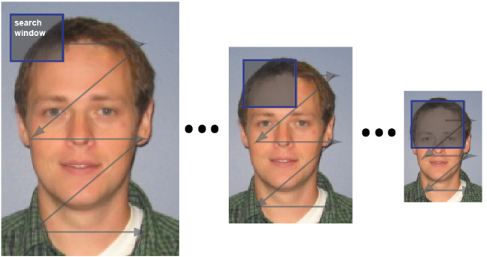
\includegraphics[width=0.8\textwidth]{Milestone2_Cascade}
\caption{Depiction of a cascade object detector, where the image is successively downsampled until the search window properly encompasses the size of object. From https://www.mathworks.com/help/vision/ref/vision.cascadeobjectdetector-system-object.html}
\label{fig:cascade}
\end{figure}


\subsection{Face and Body Segmentation}
Using the located face, the regions of the face and body can be determined. The head is important for extracting pulse rate from the facial tissues, and the body is important for extracting the respiratory rate from chest wall expansion and contraction during breathing cycles. Using the facial bounding box as the initial region, the head was defined as the face and neck, and was determined according to the following relationship:

\begin{equation}
\begin{bmatrix}
           x_h \\
           y_h \\
           w_h \\
           h_h
         \end{bmatrix} = 
\begin{bmatrix}
           x_f \\
           y_f-0.1h_f \\
           w_f \\
           1.6h_f
         \end{bmatrix}
\label{eq:bbox}
\end{equation}
where $(x,y,w,h)$ represents the ROI of the face ($\cdot _f$) and head ($\cdot _h$) based on its top-left coordinate $(x,y)$ and width and height $(w,h)$. Here, the height was extended to incorporate the neck, and was shifted upward to include the entire forehead. Then, the body ROI was defined as $I \setminus R_h$, where $I$ is the image space, $R_h$ is the head ROI, and $\setminus$ is the set difference operator.

\subsection{Absorbance Calculation}
In order to extract the blood volume signal, pixel reflectance values were converted to absorbance values:
\begin{equation}
A(x,y,t) = -\log R(x,y,t)
\end{equation}
where $R(x,y,t)$ is the reflectance value at pixel coordinate $(x,y)$ across time, and $A(x,y,t)$ is the computed absorbance signal. This relationship is derived from the Beer-Lambert law of light attenuation in absorbing media:

\begin{equation}
A = -\log \frac{I}{I_0}
\end{equation}
where $I$ and $I_0$ are the transmitted and incident illumination, respectively.

\subsection{Pulse Rate and Respiratory Rate Extraction}
The pulse rate and respiratory rate were extracting using a physiologically motivated weighted signal fusion approach. Specifically, a signal strength weight was computed for each signal representing the estimated strength of the signal as the underlying physiological (pulse or respiratory) signal. The underlying model uses the physiological prior information of signal quasi-periodicity to estimate signal strength. Normalized spectral entropy was used to model quasi-periodicity:

\begin{equation}
H(z) = \frac{F(z) \cdot \log_2 F(z)}{\log_2 N}
\end{equation}
where $N$ is the sample length, and $F(z)$ is the normalized spectral power of signal $z$ according to its Fourier transform. Note that, since entropy is a measure of randomness, quasi-periodicity is indicated by small values of entropy (i.e., low randomness). Thus, the weights for each signal were computed as inversely proportional to spectral entropy:
\begin{align}
w(x,y) = 1-H(A(x,y))
\label{eq:weights}
\end{align}

The pulse rate and respiratory rate signals were then estimated using a weighted fusion of the underlying biophotonic signals:
\begin{align}
z_{PR} = \frac{\sum_{(x_h,y_h) \in R_h} w(x_h,y_h) A(x_h,y_h)}{\sum_{(x_h,y_h) \in R_h} w(x_h,y_h)} \label{eq:z_PR} \\
z_{RR} = \frac{\sum_{(x_b,y_b) \in R_b} w(x_b,y_b) A(x_b,y_b)}{\sum_{(x_b,y_b) \in R_b} w(x_b,y_b)} \label{eq:z_RR}
\end{align}
where $R_h$ and $R_b$ are the regions of the head and body as before. The pulse rate and respiratory rate were then computed as the maximum frequency response of the respective signals.


\section{Experimental Results}
This PR and RR algorithm was evaluated using the setup discussed in Section~1. Figure~\ref{fig:face} shows the detected face using the Viola-Jones cascade object detector from the overhead view. The ROI correctly identified the face from face, excluding the neck and upper forehead. This serves as a baseline for extracting PR and RR.

\begin{figure}
\centering
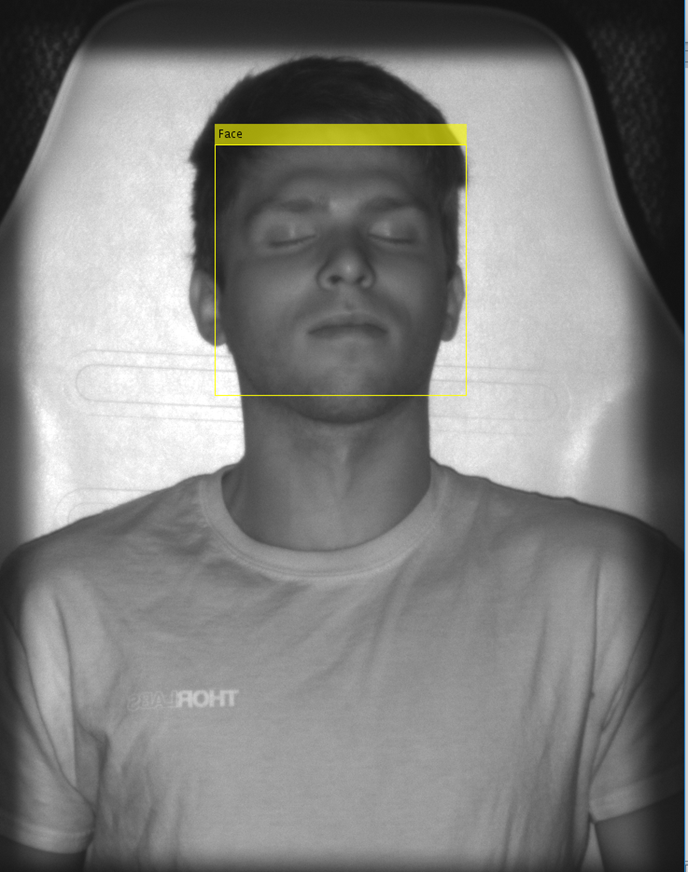
\includegraphics[width=\textwidth]{Milestone2_FaceDetect}
\caption{Frame with automatically detected facial region highlighted.}
\label{fig:face}
\end{figure}

\begin{figure}
\centering
\includegraphics[height=8in]{Milestone2_headandbody}
\caption{Visual depiction of automatically separating the head from the body for analyzing pulse rate and respiratory rate.}
\label{fig:headandbody}
\end{figure}

Note how the facial bounding box does not encompass the entire forehead and neck. This is a fundamental characteristic of the face detector, since it was trained to detect faces only. Thus, the bounding box was increased according to Equation~\ref{eq:bbox}. Then, the signal strength weights were computed according to Equation~\ref{eq:weights} in preparation for signal fusion. Figure~\ref{fig:weights} shows a visual depiction of this process. Brighter areas indicate stronger computed weights. On the left, we can see that the weights are strongest through the neck, cheek and forehead region, indicating that the algorithm identified pulsatility through the carotid and facial arteries. On the right, we can see that the weights are strongest around the chest cavity, indicating that the algorithm identified motion resulting from chest cavity expansion and contraction.

\begin{figure}
\centering
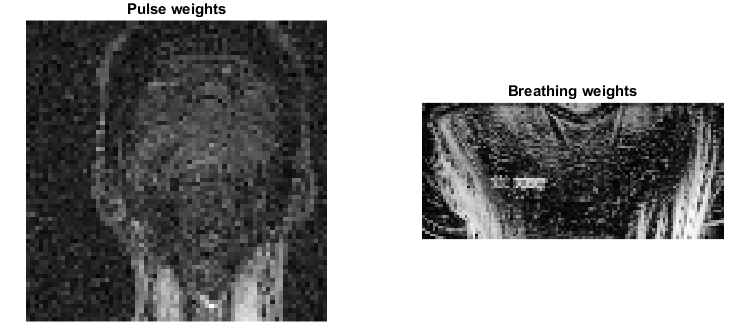
\includegraphics[width=\textwidth]{Milestone2_Weights}
\caption{Weights from frame representing the relative strength of signal at each location. The lighter the region, the stronger the weight for extracting the pulse/respiratory rate.}
\label{fig:weights}
\end{figure}

Using these weights, the pulse rate and breathing rate signals were extracted using the signal fusion method from Equation~\ref{eq:z_PR} and Equation~\ref{eq:z_RR}. The pulse rate signal shows strong arterial pulsing that is quasi periodic, resulting in a clean frequency peak at 67~bpm. Similarly, the respiratory signal is slow and quasi-periodic, resulting in a respiratory rate of 22~bpm. These were both consistent with manual observations of the participant's physiological state.

\begin{figure}
\centering
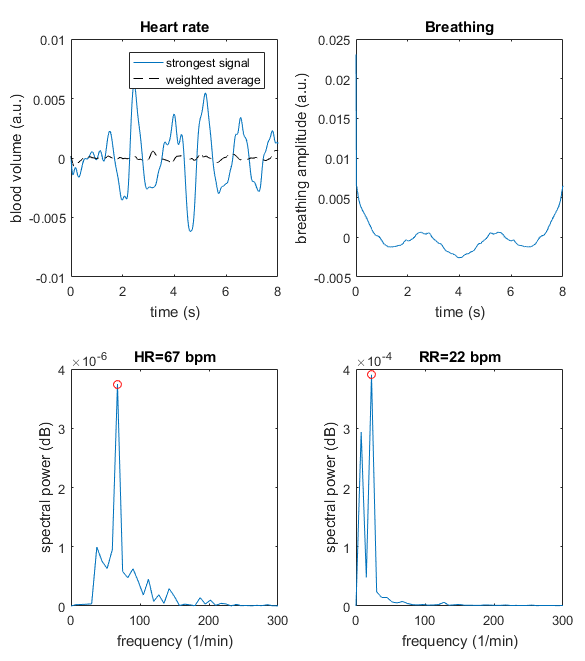
\includegraphics[width=\textwidth]{Milestone2_Signals}
\caption{Extracted pulse rate and breathing rate signals (top) and values (bottom).}
\label{fig:signals}
\end{figure}


\end{document}